% Block Def
% ---- Cavity
\def \cavityCenterX{-1.0}
\def \cavityCenterY{0.0}
\def \cavitySizeX{1.5}
\def \cavitySizeY{1}

% ---- Valve A
\def \valveACenterX{2.0}
\def \valveACenterY{2.0}
\def \valveASizeX{1.5}
\def \valveASizeY{1}

% ---- Valve B
\def \valveBCenterX{5.0}
\def \valveBCenterY{0}
\def \valveBSizeX{1.5}
\def \valveBSizeY{1}

% ---- Capacitance
\def \capacitanceCenterX{2.0}
\def \capacitanceCenterY{-2}
\def \capacitanceSizeX{2.25}
\def \capacitanceSizeY{1}

% ---- RC A
\def \rcACenterX{9.1}
\def \rcACenterY{0.0}
\def \rcASizeX{1}
\def \rcASizeY{1}

% ---- RC B
\def \rcBCenterX{13.0}
\def \rcBCenterY{0.0}
\def \rcBSizeX{1}
\def \rcBSizeY{1}

% Node Def
\def \nodeRadius{0.2}

% Ventricule
\def \ventricleCenterX{\valveACenterX}
\def \ventricleCenterY{\cavityCenterY}

% Atrium
\def \atriumCenterX{2}
\def \atriumCenterY{4}

% Proximal
\def \proximalCenterX{7.25}
\def \proximalCenterY{0.0}

% Distal
\def \distalCenterX{11}
\def \distalCenterY{0.0}

% Venous
\def \venousCenterX{15}
\def \venousCenterY{0.0}

% Flux Def
\def \fluxShift{1.0}

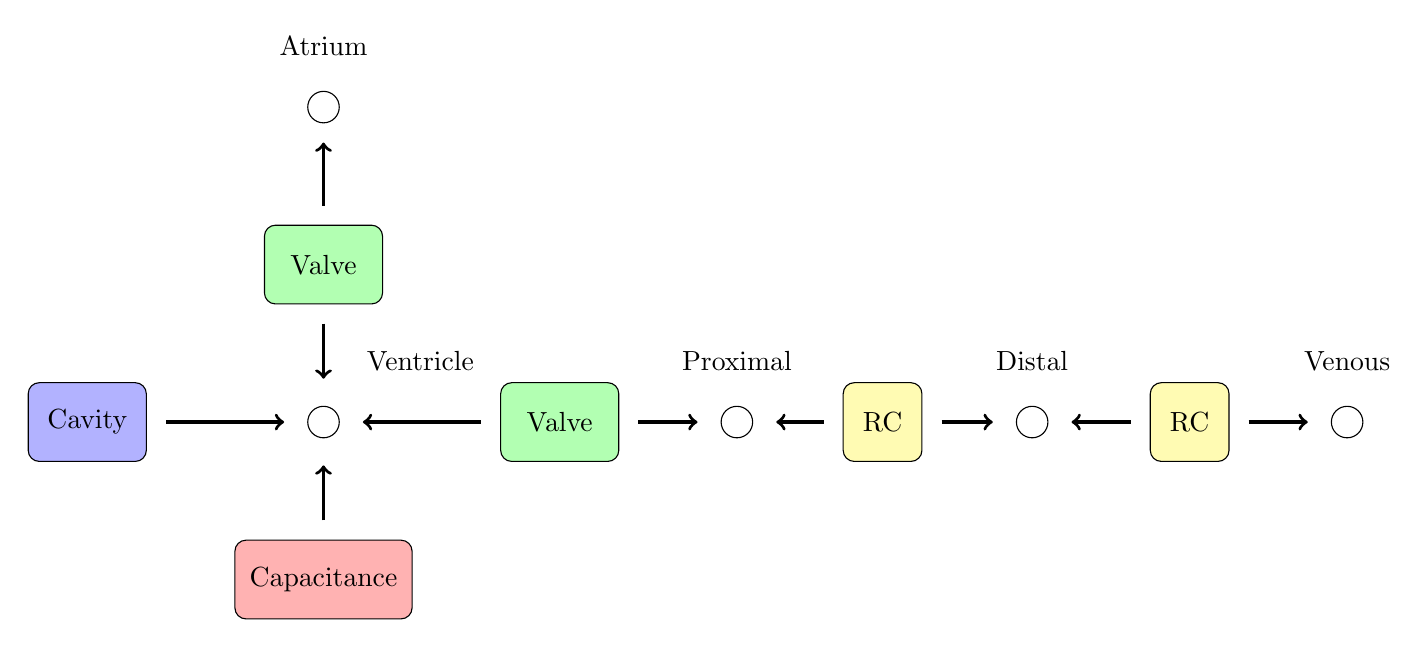
\begin{tikzpicture}
% ---- Nodes circles
% ---- Ventricle
\draw (\ventricleCenterX, \ventricleCenterY) circle [radius = \nodeRadius] node [anchor=south, xshift=35, yshift = 15] {Ventricle};
% ---- Atrium
\draw (\atriumCenterX, \atriumCenterY) circle [radius = \nodeRadius] node [anchor=south, yshift = 15] {Atrium};
% ---- Proximal
\draw (\proximalCenterX, \proximalCenterY) circle [radius = \nodeRadius] node [anchor=south, yshift = 15] {Proximal};
% ---- Distal
\draw (\distalCenterX, \distalCenterY) circle [radius = \nodeRadius] node [anchor=south, yshift = 15] {Distal};
% ---- Venous
\draw (\venousCenterX, \venousCenterY) circle [radius = \nodeRadius] node [anchor=south, yshift = 15] {Venous};

% ---- Blocks boxes
% ---- Cavity
\filldraw[rounded corners, fill=blue!30] (\cavityCenterX - \cavitySizeX / 2, \cavityCenterY - \cavitySizeY / 2) rectangle (\cavityCenterX + \cavitySizeX / 2, \cavityCenterY + \cavitySizeY / 2) node[pos=.5] {Cavity};
% ---- Valve A
\filldraw[rounded corners, fill=green!30] (\valveACenterX - \valveASizeX / 2, \valveACenterY - \valveASizeY / 2) rectangle (\valveACenterX + \valveASizeX / 2, \valveACenterY + \valveASizeY / 2) node[pos=.5] {Valve};
% ---- Valve B
\filldraw[rounded corners, fill=green!30] (\valveBCenterX - \valveBSizeX / 2, \valveBCenterY - \valveBSizeY / 2) rectangle (\valveBCenterX + \valveBSizeX / 2, \valveBCenterY + \valveBSizeY / 2) node[pos=.5] {Valve};
% ---- Capacitance
\filldraw[rounded corners, fill=red!30] (\capacitanceCenterX - \capacitanceSizeX / 2, \capacitanceCenterY - \capacitanceSizeY / 2) rectangle (\capacitanceCenterX + \capacitanceSizeX / 2, \capacitanceCenterY + \capacitanceSizeY / 2) node[pos=.5] {Capacitance};
% ---- RC 1
\filldraw[rounded corners, fill=yellow!30] (\rcACenterX - \rcASizeX / 2, \rcACenterY - \rcASizeY / 2) rectangle (\rcACenterX + \rcASizeX / 2, \rcACenterY + \rcASizeY / 2) node[pos=.5] {RC};
% ---- RC 2
\filldraw[rounded corners, fill=yellow!30] (\rcBCenterX - \rcBSizeX / 2, \rcBCenterY - \rcBSizeY / 2) rectangle (\rcBCenterX + \rcBSizeX / 2, \rcBCenterY + \rcBSizeY / 2) node[pos=.5] {RC};

% Flux
\draw [very thick][->] (\cavityCenterX + 1.0, 0) -- (\ventricleCenterX - 0.5, 0);
\draw [very thick][->] (\ventricleCenterX, \valveACenterY - 0.75) -- (\ventricleCenterX, \ventricleCenterY + 0.55);
\draw [very thick][->] (\ventricleCenterX, \capacitanceCenterY + 0.75) -- (\ventricleCenterX, \ventricleCenterY - 0.55);
\draw [very thick][->] (\ventricleCenterX, \valveACenterY + 0.75) -- (\ventricleCenterX, \atriumCenterY - 0.45);
\draw [very thick][<-] (\ventricleCenterX + 0.5, 0) -- (\valveBCenterX - 1.0, 0);
\draw [very thick][->] (\valveBCenterX + 1.0, 0) -- (\proximalCenterX - 0.5, 0);
\draw [very thick][<-] (\proximalCenterX + 0.5, 0) -- (\rcACenterX - 0.75, 0);
\draw [very thick][->] (\rcACenterX + 0.75, 0) -- (\distalCenterX - 0.5, 0);
\draw [very thick][<-] (\distalCenterX + 0.5, 0) -- (\rcBCenterX - 0.75, 0);
\draw [very thick][->] (\rcBCenterX + 0.75, 0) -- (\venousCenterX - 0.5, 0);
\end{tikzpicture}